	\documentclass[11pt]{book}
	
	\usepackage{amsfonts,amsthm, bm,amsmath, bbm,amssymb,mathtools}
	\usepackage{fullpage}
	\usepackage{tikz, pgfplots} % added for Lecture 2	
	\usepackage{float}  % added for Lecture 8
	
	\newtheorem{theorem}{Theorem}[chapter]
	\newtheorem{lemma}[theorem]{Lemma}
	
	\theoremstyle{definition}
	\newtheorem{definition}[theorem]{Definition}
	\newtheorem{example}[theorem]{Example}
	\newtheorem{xca}[theorem]{Exercise}
	\newtheorem{corollary}[theorem]{Corollary}  % added for Lecture 5
	\newtheorem{proposition}{Proposition}[section]  % added for Lecture 6
		
	\theoremstyle{remark}
	\newtheorem{remark}[theorem]{Remark}
	
	\numberwithin{section}{chapter}
	\numberwithin{equation}{chapter}
	
	\makeindex
	
	\def\lectureformat{1}
	\usepackage{color}
\usepackage{lipsum}

\ifnum\lectureformat=1
\newcommand{\metadata}[3]
{
	\newpage
	
	\def\lectureID{#1}
	
	\setcounter{chapter}{\lectureID}

%	\draftnotice
	
	\begin{center}
		\bf\large CS229M/STATS214: Machine Learning Theory
	\end{center}
	
	\noindent
	Lecturer: Tengyu Ma   %%% FILL IN LECTURER (if not RS)
	\hfill
	Lecture \# \lectureID              %%% FILL IN LECTURE NUMBER HERE
	\\
	Scribe: #2                  %%% FILL IN YOUR NAME HERE
	\hfill
	#3           %%% FILL IN LECTURE DATE HERE
	
	\noindent
	\rule{\textwidth}{1pt}
	
	\medskip
}
\else 
\newcommand{\metadata}[3]{}
\fi

\newcommand*\circled[1]{\tikz[baseline=(char.base)]{
	\node[shape=circle,draw,inner sep=2pt] (char) {#1};}}

\DeclareMathOperator*{\Exp}{\mathbb{E}}
\DeclareMathOperator*{\argmin}{\textup{argmin}}
\DeclareMathOperator*{\argmax}{\textup{argmax}}

\newcommand{\Cov}{\operatorname{Cov}}
\newcommand{\KL}{\operatorname{KL}}
\newcommand{\margin}{\text{margin}}
\newcommand{\poly}{\operatorname{poly}}
\newcommand{\sd}{\operatorname{sd}}
\newcommand{\sgn}{\text{sgn}}
\newcommand{\tr}{\operatorname{tr}}
\newcommand{\Var}{\operatorname{Var}}

\newcommand{\err}{\ell_{\textup{0-1}}}
\newcommand{\Err}{L_{\textup{0-1}}}
\newcommand{\thetaerm}{\theta_{\textup{ERM}}}
\newcommand{\hatL}{\widehat{L}}
\newcommand{\tilO}{\widetilde{O}}
\newcommand{\iid}{\overset{\textup{iid}}{\sim}}
\newcommand\defeq{\stackrel{\mathclap{\tiny \mbox{$\Delta$}}}{=}}

\newcommand{\norm}[1]{\|#1\|}
\newcommand{\Norm}[1]{\left\|#1\right\|}
\renewcommand{\l}{\left}
\renewcommand{\r}{\right}
\newcommand{\rbr}[1]{\left(#1\right)}
\newcommand{\sbr}[1]{\left[#1\right]}
\newcommand{\cbr}[1]{\left\{#1\right\}}
\newcommand{\abs}[1]{\left\lvert#1\right\rvert}
\newcommand{\inprod}[1]{\left\langle#1\right\rangle}

\newcommand{\al}[1]{
	\begin{align}
	#1
	\end{align}
}

\renewcommand{\sp}[1]{^{(#1)}}

\newcommand{\cA}{\mathcal A}
\newcommand{\cB}{\mathcal B}
\newcommand{\cC}{\mathcal C}
\newcommand{\cD}{\mathcal D}
\newcommand{\cE}{\mathcal E}
\newcommand{\cF}{\mathcal F}
\newcommand{\cG}{\mathcal G}
\newcommand{\cH}{\mathcal H}
\newcommand{\cI}{\mathcal I}
\newcommand{\cJ}{\mathcal J}
\newcommand{\cK}{\mathcal K}
\newcommand{\cL}{\mathcal L}
\newcommand{\cM}{\mathcal M}
\newcommand{\cN}{\mathcal N}
\newcommand{\cO}{\mathcal O}
\newcommand{\cP}{\mathcal P}
\newcommand{\cQ}{\mathcal Q}
\newcommand{\cR}{\mathcal R}
\newcommand{\cS}{\mathcal S}
\newcommand{\cT}{\mathcal T}
\newcommand{\cU}{\mathcal U}
\newcommand{\cV}{\mathcal V}
\newcommand{\cW}{\mathcal W}
\newcommand{\cX}{\mathcal X}
\newcommand{\cY}{\mathcal Y}
\newcommand{\cZ}{\mathcal Z}

\newcommand{\bbB}{\mathbb B}
\newcommand{\bbS}{\mathbb S}
\newcommand{\bbR}{\mathbb R}
\newcommand{\bbZ}{\mathbb Z}
\newcommand{\bbI}{\mathbb I}
\newcommand{\bbQ}{\mathbb Q}
\newcommand{\bbP}{\mathbb P}
\newcommand{\bbE}{\mathbb E}
\newcommand{\bbN}{\mathbb N}

\newcommand{\E}{\mathbb{E}}
\newcommand{\N}{\mathbb{N}}
\newcommand{\R}{\bbR}
\newcommand{\Z}{\mathbb{Z}}


% for course staff to edit or comment
\def\shownotes{1}  %set 1 to show author notes
\ifnum\shownotes=1
\newcommand{\authnote}[2]{[#1: #2]}
\else
\newcommand{\authnote}[2]{}
\fi
\newcommand{\tnote}[1]{{\color{blue}\authnote{TM}{#1}}}

% for long term comments 
\def\shownotes{0}  %set 1 to show author notes
\ifnum\shownotes=1
\newcommand{\authnotelong}[2]{[#1: #2]}
\else
\newcommand{\authnotelong}[2]{}
\fi
\newcommand{\tnotelong}[1]{{\color{blue}\authnotelong{TM}{#1}}}
	\begin{document}
	
	\frontmatter
	
	\mainmatter
	\let\sec\section
	\let\subsec\subsection
	
	\newcommand{\secwarning}[1]{
		{	
			\color{red}
			$\backslash$section and $\backslash$subsection are disallowed, please use 	$\backslash$sec and $\backslash$subsec instead
		}
	}
	\let\section\secwarning
	\let\subsection\secwarning
	
	
	\newcommand{\draftnotice}{\vbox to 0.25in{\noindent
			\raisebox{0.6in}[0in][0in]{\makebox[\textwidth][r]{\it
					DRAFT --- a final version will be posted shortly}}}
		\vspace{-.25in}\vspace{-\baselineskip}
	}
	
	%\section{}
	 % reset section counter
\setcounter{section}{0}
\metadata{8}{David Lin and Jinhui Wang}{Feb.~8th, 2021}


%*****************************************************************************
\sec{Review and overview}
In the previous lecture, we derived explicit Rademacher complexity bounds for linear models with weights bounded in $\ell_1$ and $\ell_2$ norms. To recap, we proved:

\begin{theorem}\label{lec8:thm:thm7.1}
Let $\mathcal{H}=\left\{x \mapsto\langle w, x\rangle \mid w \in \mathbb{R}^{d},\|w\|_{2} \leq B\right\}$ for some constant $B>0 .$ Moreover, assume $\mathbb{E}_{x \sim P}\left[\|x\|_{2}^{2}\right] \leq C^{2},$ where $P$ is some distribution and $C>0$ is a constant. Then
\begin{equation}
R_{S}(\mathcal{H}) \leq \frac{B}{n} \sqrt{\sum_{i=1}^{n}\left\|x\sp{i}\right\|_{2}^{2}}, \quad\text{and}\quad 
R_n(\mathcal{H}) \leq \frac{BC}{\sqrt{n}}.
\end{equation}
\end{theorem}

\begin{theorem}\label{lec8:thm:thm7.3}
Let $\mathcal{H}=\left\{x \mapsto\langle w, x\rangle \mid w \in \mathbb{R}^{d},\|w\|_{1} \leq B\right\}$ for some constant $B>0$. Moreover, assume $\left\|x\sp{i}\right\|_{\infty} \leq C$ for some constant $C>0$ and all points in $S=\left\{x\sp{i}\right\}_{i=1}^{n} \subset \mathbb{R}^{d} .$ Then
\begin{equation}
R_{S}(\mathcal{H}) \leq B C \sqrt{\frac{2 \log (2 d)}{n}}.
\end{equation}
\end{theorem}

We also derived a crude bound for a two-layer neural network $f_{\theta}: \mathbb{R}^d \to \mathbb{R}$ defined by $f_{\theta}(x) = w^\top \phi (Ux)$. Here, $U = \begin{pmatrix}
u_1^\top \\
\vdots \\
u_m^\top
\end{pmatrix} \in \mathbb{R}^{m \times d}$ and $w \in \mathbb{R}^m$ correspond to the weight matrices in the first and second layers of the neural network respectively while $\phi(z) = \max(z, 0)$ is the ReLU activation function taken elementwise. (We can think of the network as being parameterized by the pair $\theta = (w, U)$.) For this set-up, we showed:

\begin{theorem}\label{lec8:thm:thm7.5}
For some constants $B_{w}>0$ and $B_{u}>0$, let
\begin{equation}
\mathcal{H}=\left\{f_{\theta} \mid\|w\|_{2} \leq B_{w},\left\|u_{i}\right\|_{2} \leq B_{u}, \forall i \in\{1,2, \ldots, m\}\right\}, \label{lec8:eqn:old-bound-class}
\end{equation}
and suppose $\mathbb{E}\left[\|x\|_{2}^{2}\right] \leq C^{2} .$ Then
\begin{equation}
R_{n}(\mathcal{H}) \leq 2 B_{w} B_{u} C \sqrt{\frac{m}{n}}.
\end{equation}
\end{theorem}

This upper bound is undesirable since it grows with the number of neurons $m$, contradicting empirical observations of the generalization error decreasing with $m$. Today, we will complete the proof of a refined upper bound that is non-increasing with $m$ by leveraging a finer definition of complexity $C(\theta)$. Subsequently, we discuss implications of this new theorem before transitioning to a new method of bounding Rademacher complexities by covering the output space.

%*****************************************************************************

\sec{Refined bound for two-layer neural networks}

A recurring theme in subsequent proofs will be the functional invariance of two-layer neural networks under a class of rescaling transformations. The key ingredient will be the \textit{positive homogeneity} of the ReLU function, i.e.
\begin{equation}
\alpha \phi(x) = \phi(\alpha x) \qquad \forall \alpha > 0.
\end{equation}
This implies that for any $\lambda_i > 0$ ($i = 1, \dots, m$), the transformation $\theta = \{(w_i, u_i)\}_{1 \leq i \leq m} \mapsto \theta' = \{(\lambda_i w_i,  u_i / \lambda_i )\}_{1 \leq i \leq m}$ has no net effect on the neural network's functionality (i.e. $f_{\theta} = f_{\theta'}$) since 
\begin{equation}
w_i\cdot \phi \left(u_i^\top x\sp i \right) = (\lambda_i w_i) \cdot \phi\l(\l( \frac{u_i}{\lambda_i}\r)^\top x\sp i\r).   
\end{equation}
In light of this, we devise a new complexity measure $C(\theta)$ that is also invariant under such transformations and use it to prove a better bound for the Rademacher complexity. This positive homogeneity property is absent in the (implicit) complexity measure used in the hypothesis class \eqref{lec8:eqn:old-bound-class} of Theorem \ref{lec8:thm:thm7.5}. 

\begin{theorem}\label{lec8:thm:thm-improved-nn-rc}
$\operatorname{Let} C(\theta)=\sum_{j=1}^{m}\left|w_{j}\right|\left\|u_{j}\right\|_{2},$ and for some constant $B_{C}>0$ consider the hypothesis class
\begin{equation}
\mathcal{H}=\left\{f_{\theta} \mid C(\theta) \leq B_{C}\right\}.
\end{equation}
If $\left\|x\sp{i}\right\|_{2} \leq C$ for all $i \in\{1, \ldots, n\},$ then
\begin{equation}
R_{S}(\mathcal{H}) \leq \frac{2 B_{C} C}{\sqrt{n}}.
\end{equation}
\end{theorem}

\begin{proof}
Due to the positive homogeneity of the ReLU function $\phi$, it will be useful to define the $\ell_2$-normalized weight vector $\bar{u}_j := u_j / \norm{u_j}_2$ so that $\phi\left(u_j^T x\right) = \norm{u_j}_2 \cdot \phi(\bar{u}_j^T x)$. The empirical Rademacher complexity satisfies
\allowdisplaybreaks
\al{
R_S(\cH) &= \frac{1}{n}\E_{\sigma}\left[ \sup_{\theta} \sum_{i=1}^n \sigma_i f_{\theta}\left(x\sp{i}\right) \right] \\
&= \frac{1}{n}\E_{\sigma}\left[ \sup_{\theta} \sum_{i=1}^n \sigma_i \left[\sum_{j=1}^m w_j \phi\left(u_j ^ T x\sp{i}\right) \right] \right] &&\text{(by dfn of $f_\theta$)} \\
&=  \frac{1}{n}\E_{\sigma}\left[ \sup_{\theta} \sum_{i=1}^n \sigma_i \left[\sum_{j=1}^m w_j \norm{u_j}_2  \phi\left(\bar{u}_j ^ T x\sp{i}\right) \right] \right]  
    && \text{(by positive homogeneity of $\phi$)}\\
&= \frac{1}{n}\E_{\sigma}\left[ \sup_{\theta}  \sum_{j=1}^m w_j \norm{u_j}_2 \left[ \sum_{i=1}^n \sigma_i  \phi\left(\bar{u}_j ^ T x\sp{i}\right) \right] \right] \\ 
&\leq \frac{1}{n}\E_{\sigma}\left[ \sup_{\theta}  \sum_{j=1}^m |w_j| \norm{u_j}_2 \max_{k \in [n]}\left| \sum_{i=1}^n \sigma_i  \phi\left(\bar{u}_k ^ T x\sp{i}\right) \right| \right] && \l(\because \sum_j \alpha_j \beta_j \leq \sum_j |\alpha_j| \max_{k} |\beta_k|\r) \\ 
&\leq \frac{B_C}{n} \E_{\sigma}\sbr{ \sup_{\theta = (w, U)} \max_{k \in [n]} \left| \sum_{i=1}^n \sigma_i  \phi\left(\bar{u}_k ^ T x\sp{i}\right) \right| } && \text{( $\because C(\theta) \leq B_C$)} \\
&=  \frac{B_C}{n} \E_{\sigma}\sbr{ \sup_{\bar{u}: \norm{\bar{u}}_2 = 1} \left| \sum_{i=1}^n \sigma_i  \phi\left(\bar{u} ^ T x\sp{i}\right) \right| } \\
&\le \frac{B_C}{n} \E_{\sigma}\sbr{ \sup_{\bar{u}: \norm{\bar{u}}_2 \le 1} \left| \sum_{i=1}^n \sigma_i  \phi\left(\bar{u} ^ T x\sp{i}\right) \right| } \\
&\le \frac{2B_C}{n}  \E_{\sigma}\sbr{ \sup_{\bar{u}: \norm{\bar{u}}_2 \le 1} \sum_{i=1}^n \sigma_i  \phi\left(\bar{u} ^ T x\sp{i}\right) } && \text{(see Lemma \ref{lec8:lemma:absfortwo})} \\
&= 2B_C R_S(\cH '),
}
where $\cH' = \l\{x \mapsto \phi(\bar{u}^T x) :  \bar{u} \in \mathbb{R}^d, \norm{\bar{u}}_2 \leq 1 \r\}$. By Talagrand's lemma, since $\phi$ is $1$-Lipschitz, $R_S(\cH') \leq R_S(\cH'')$ where  $\cH'' = \l\{x \mapsto \bar{u}^T x :  \bar{u} \in \mathbb{R}^d, \norm{\bar{u}}_2 \leq 1 \r\}$ is a linear hypothesis space. Using $R_S(\cH'') \leq \frac{C}{\sqrt{n}}$ by Theorem \ref{lec8:thm:thm7.1} then concludes the proof.

\end{proof}

\begin{remark}
This refined upper bound is much stronger than Theorem \ref{lec8:thm:thm7.5} since it does not increase with the number of neurons $m$. Notably, we can analyse the $m \to \infty$ limit and still hope to obtain a non-vacuous bound. Intuitively, this is because the network has a fixed ``budget'' $B_C$ that it is allowed to distribute among an arbitrary number of neurons.
\end{remark}


We complete the proof by deriving the Lemma \ref{lec8:lemma:absfortwo} used in the second last inequality. Notably, the lemma's assumption holds in the current context, since
\al{
\sup_{\theta} \langle \sigma, f_{\theta}(x) \rangle = \sup_{\bar{u}: \norm{\bar{u}}_2 \leq 1} 
\sum_{i=1}^n \sigma_i \phi \l(\bar{u}^T x\sp i \r)  \geq 0.
}
since one can take $\bar{u} = 0$ for any $\sigma = (\sigma_1, \dots, \sigma_n)$.

\begin{lemma}\label{lec8:lemma:absfortwo}
Let $\sigma = (\sigma_1, ..., \sigma_n)$ and $f_{\theta}(x) = \l(f_{\theta}\l(x\sp{1}\r), ...,  f_{\theta}\l(x\sp{n} \r)\r)$. Suppose that for any $\sigma \in \{\pm 1\}^n$, $\sup_{\theta} \langle \sigma, f_{\theta}(x) \rangle \geq 0$. Then, 
\begin{equation}
\mathbb{E}_{\sigma}\l[ \sup_{\theta}  \l | \langle \sigma, f_{\theta}(x) \rangle \r|  \r] \leq 2 \mathbb{E}_{\sigma}\l[ \sup_{\theta}  \langle \sigma, f_{\theta}(x) \rangle   \r].
\end{equation}
\end{lemma}

\begin{proof}
Letting $\phi$ be the ReLU function, the lemma's assumption implies that $\sup_{\theta} \phi\left(\langle \sigma, f_{\theta}(x) \rangle\right) = \sup_{\theta}\langle \sigma, f_{\theta}(x) \rangle$ for any $\sigma \in \{\pm 1\}^n$. Observing that $|z| = \phi(z) + \phi(-z)$, 
\begin{align}
\sup_{\theta} \abs{\inprod{ \sigma, f_{\theta}(x) }}%
&= \sup_{\theta} \left[ \phi \l(\inprod{ \sigma, f_{\theta}(x) } \r) + \phi \l(\inprod{-\sigma, f_{\theta}(x) } \r)\right] \\
&\le \sup_{\theta}  \phi \l(\inprod{ \sigma, f_{\theta}(x) } \r) +  \sup_{\theta}  \phi \l(\inprod{-\sigma, f_{\theta}(x) } \r)  \\
&= \sup_{\theta} \inprod{ \sigma, f_{\theta}(x) } +  \sup_{\theta}  \inprod{-\sigma, f_{\theta}(x) }. 
\end{align}
Taking the expectation over $\sigma$ (and noting that $\sigma \overset d = -\sigma$), we get the desired conclusion.
\end{proof}


\sec{Consequences of refined bound}
In this section, we discuss practical implications of the refined neural network bound. 

\subsec{Connection to $\ell_2$ regularization}

Recall that margin theory yields
\begin{equation}
\text{for all } \theta, \quad \Err(\theta) \leq \frac{2R_S(\cH)}{\gammamin} + \tilO\l(\sqrt{\frac{\log \l( 2 / \delta \r)}{n}}\r), \label{lec8:eqn:margin-bound}
\end{equation}
with probability at least $1 -\delta$. Thus, Theorem \ref{lec8:thm:thm-improved-nn-rc} motivates us to minimize $\frac{R_S(\cH)}{\gammamin}$ by regularizing $C(\theta)$. Concretely, this can be formulated as the optimization problem 
\al{
\text{minimize} & \qquad C(\theta) = \sum_{j=1}^m |w_j|\cdot \norm{u_j}_2 \nonumber \tag{I} \label{lec8:eqn:opt1} \\ 
\text{subject to} & \qquad \gammamin(\theta)\ge 1, \nonumber
}
or equivalently,
\al{
\text{maximize} & \qquad \gammamin(\theta) \nonumber \tag{II} \label{lec8:eqn:opt2} \\ 
\text{subject to} & \qquad C(\theta)\le 1. \nonumber
}

At first glance, the above seems orthogonal to techniques used in practice. However, it turns out that the optimal neural network from \eqref{lec8:eqn:opt1} is functionally equivalent to that of the new problem:
\al{
\text{minimize} & \qquad C_{\ell_2}(\theta) = \frac{1}{2}\sum_{j=1}^m |w_j|^2 + \frac{1}{2}\sum_{j=1}^m \norm{u_j}_2^2 \nonumber \tag{I*} \label{lec8:eqn:opt1star} \\ 
\text{subject to} & \qquad \gammamin(\theta)\ge 1. \nonumber
}
This is a simple consequence of the positive homogeneity of $\phi$. For any scaling factor $\lambda=(\lambda_1, \dots, \lambda_m)\in \R_+^m$, the rescaled neural network $\theta_\lambda := \{(\lambda_i w_i, u_i/\lambda_i)\}$ has the same functionality as the original neural network $\theta = \{w_i, u_i \}$ (i.e. it achieves the same $\gammamin$). Thus, 
\al{
\min_{\theta} C_{\ell_2}(\theta) &= \min_{\theta} \min_{\lambda} \rbr{ \frac{1}{2}\sum_{j=1}^m \lambda_j^2 |w_j|^2 + \frac{1}{2}\sum_{j=1}^m \lambda_j^{-2}\norm{u_j}_2^2 }\\
&= \min_{\theta}  \sum_{j=1}^m |w_j|\cdot \norm{u_j}_2 \\
&= \min_{\theta}  C(\theta)
}

where we have used the equality case of the AM-GM inequality, attainable by $\lambda_j^* = \sqrt{\frac{\norm{u_j}_2}{|w_j|}}$, in the second step. This equality case also shows that $\theta^* = \{(w_i, u_i ) \}$ is the optimal solution of \eqref{lec8:eqn:opt1} if and only if $\hat{\theta}^* = \theta_{\lambda^*}$ is the optimal solution of \eqref{lec8:eqn:opt1star}---proving that $\hat{\theta}^*$ and $\theta^*$ are functionally equivalent since they only differ by a positive scale factor. 


This connects our $C(\theta)$ regularization to $\ell_2$-norm penalties that are more prevalent in practice. In retrospect, we see this equivalence is essentially due to the positive homogeneity of the neural network which ``homogenizes'' any inhomogeneous objective such as $C_{\ell_2}$. Hence, we can just deal with $C(\theta)$ which is transparently homogeneous.

\subsec{Stable generalization bound in $m$} 

Next, we show that the generalization bound given by Theorem \ref{lec8:thm:thm-improved-nn-rc} does not deteriorate with the network width (number of neurons) $m$, which is consistent with experimental results. To this end, the perspective of \eqref{lec8:eqn:opt2} enables us to isolate all dependencies of $m$ in $\gammamin$. Letting $\widehat \theta_m$ denote the minimizer of program \eqref{lec8:eqn:opt2} with width $m$ and defining optimal value $\gamma_m^* = \gammamin\l(\widehat \theta_m\r)$, we can rewrite the margin bound \eqref{lec8:eqn:margin-bound} as 
\begin{equation}
L(\widehat \theta_m) \le \frac{4C}{\sqrt{n}} \cdot \frac{1}{\gamma_m^*} + \text{(lower-order terms)},
\end{equation}
where all dependencies on $m$ are now contained in $\gamma_m^*$. Hence, to show that this bound does not worsen as $m$ grows, we just have to show that $\gamma_m^*$ is non-decreasing in $m$. This is intuitively the case since a neural network of width $m+1$ contains one of width $m$ under the same complexity constraints. The following theorem formalizes this hunch:

\begin{theorem}
Let $\gamma_m^*$ be the minimum margin obtained by solving \eqref{lec8:eqn:opt2} with a two-layer neural network of width $m$. Then $\gamma_m^* \leq \gamma_{m+j}^*$ for all positive integers $j$.
\end{theorem}

\begin{proof}
Suppose $\theta = \{(w_i, u_i)\}_{1 \leq i \leq m}$ is a two-layer neural network of width $m$ satisfying $C(\theta)\le 1$. Then we may construct a neural network $\widetilde \theta = \{(\tilde w_i, \tilde u_i)\}_{1 \leq i \leq m+1}$ of width $m+1$ by simply taking
\al{
(\widetilde w_i, \widetilde u_i) = \begin{cases}
(w_i, u_i) & i\le m, \\
(0,0) & \text{otherwise}
\end{cases}
}
$\widetilde \theta$ is functionally equivalent to $\theta$ and $C(\widetilde \theta) = C(\theta) \le 1$. This means maximizing $\gammamin$ over $\{C(\widetilde \theta): \widetilde \theta\text{ of width }m+1\}$ should give no lower of a value than the maximum of $\gammamin$ over $\{C(\theta): \theta\text{ of width }m\}$.
\end{proof}

\subsec{Equivalence to an $\ell_1$-SVM in $m \to \infty$ limit}

Since $\gamma_m^*$ is non-decreasing in $m$, quantity 
\begin{equation}
\gamma_\infty ^* = \lim_{m\to \infty } \gamma_m^*
\end{equation}
is well-defined. The next interesting fact is that in this $m \to \infty$ limit, $\gamma_{\infty}^*$ of the two-layer neural network is equivalent to the minimum margin of an $\ell_1$-SVM. As a brief digression, we recap the formulation of $\ell_p$-SVMs and discuss the importance of $\ell_1$-SVMs in particular.

Since a collection of data points with binary class labels may not be a priori separable, a \textit{kernel model} first transforms an input $x$ to $\Phi(x)$ where $\Phi: \mathbb{R}^d \to \mathcal{G}$ is known as the \textit{feature map}. The model then seeks a separating hyperplane in this new (extremely high-dimensional) feature space $\mathcal{G}$, parameterized by a vector $\mu$ pointing from the origin to the hyperplane. The prediction of the model on an input $x$ is then a decision score that quantifies $\Phi(x)$'s displacement with respect to the hyperplane:
\begin{equation}
g_{\mu, \Phi}(x) := \l\langle \mu, \Phi(x) \r\rangle.
\end{equation}
Motivated by margin theory, it is desirable to seek the maximum-margin hyperplane under a constraint on $\mu$ to guarantee the generalizability of the model. In particular, a kernel model with an $\ell_p$-constraint seeks to solve the following program:
\al{
\text{maximize} & \qquad \gamma_{min} \coloneqq \min_{i \in [n]} y\sp{i}\langle \mu, \Phi(x\sp{i}) \rangle \\ 
\text{subject to} & \qquad \norm{\mu}_p \le 1. \nonumber
}
Observe that both the prediction and optimization of the feature model only rely on inner products in $\mathcal{G}$. The ingenuity of the SVM is to choose maps $\Phi$ such that $K(x, x') = \l\langle \Phi(x), \Phi(x') \r\rangle$ can be directly computed in terms of $x$ and $x'$ in the original space $\mathbb{R}^d$, thereby circumventing the need to perform expensive inner products in the large space $\mathcal{G}$. Remarkably, this ``kernel trick'' enables us to even operate in an implicit, infinite-dimensional $\mathcal{G}$. 

The case of $p=1$ is particularly useful in practice as $\ell_1$-regularization generally produces sparse feature weights (the constrained parameter space is a polyhedron and the optimum tends to lie at one of its vertices). Hence, $\ell_1$-regularization is an important feature selection method when one expects only a few dimensions of $\cG$ to be significant. Unfortunately, the $\ell_1$-SVM is not kernelizable due to the kernel trick relying on $\ell_2$-geometry, and is hence infeasible to implement. However, our next theorem shows that a two-layer neural network can approximate a particular $\ell_1$-SVM in the $m \to \infty$ limit (and in fact, for finite $m$). For the sake of simplicity, we sacrifice rigor in defining the space $\mathcal{G}$ and convey the main ideas.

\begin{theorem}\label{lec8:thm:thm8.5}
Define the feature map $\phirelu: \mathbb{R}^d \to \mathcal{G}$ such that $x$ is mapped to $\phi(u^\top x)$ for all vectors $u$ on the $d-1$-dimensional sphere $\mathcal{S}^{d-1}$. Informally, 
$$\phirelu(x) := \begin{bmatrix} \vdots \\ \phi(u^\top x) \\ \vdots \end{bmatrix}_{u\in S^{d-1}}$$
is an ``infinite-dimensional vector'' that contains an entry $\phi(u^T x)$ for each vector $u \in \mathcal{S}^{d-1}$, and we let $\phirelu(x)[u]$ denote the ``$u$''-th entry of this vector. Noting that $\mathcal{G}$ is the space of functions which can be indexed by $u \in S^{d-1}$, the inner product structure on $\mathcal{G}$ is defined by $\langle f, g \rangle = \int_{S^{d-1}} f[u]g[u] du$.

Under this set-up, we have
\begin{equation}
\gamma_{\infty}^* = \gamma_{\ell_1}^*,
\end{equation}
where $\gamma_{\ell_1}^*$ is the minimum margin of the optimized $\ell_1$-SVM with $\Phi = \phirelu$.
\end{theorem}

\begin{proof}

We will only prove the $\gamma_{\infty}^* \leq \gamma_{\ell_1}^*$ direction. (The $\gamma_{\infty}^* \geq \gamma_{\ell_1}^*$ direction is essentially the same but requires slightly more work.)

Suppose $\gamma_\infty^*$ is obtained by network weights $(w_1,w_2, \cdots), (u_1, u_2, \cdots)$ where $w_i\in \R, u_i\in \R^d$ (there is a slight subtlety here to be rectified later). Define renormalized versions of $\{w_i\}$ and $\{u_i\}$:
\begin{equation}
\widetilde w_i := w_i\cdot \norm{u_i}_2, \qquad \overline u_i := \frac {u_i} {\norm{u_i}_2}.   
\end{equation}
Note that $\{(\widetilde w_i, \overline u_i)\}$ has the same functionality (and also the same complexity measure $C(\theta)$, margin, etc.) as that of $\{(w_i,u_i)\}$, but now $\overline u_i$ has unit $\ell_2$-norm (i.e. $\bar{u}_i \in \mathcal{S}^{d-1}$). Thus, $\phi(\overline u_i ^\top x)$ can be treated as a feature in $\cG$ and we can construct an equivalent $\ell_1$-SVM (denoted by $\mu$) such that $\widetilde w_i$ is the coefficient of $\mu$ associated with that feature. Since $\widetilde w_i$ must only be ``turned on' at $\overline u_i $, we have 
\al{
\mu[u] = \sum_{i \in \mathcal{S}^{d-1}} \tilde{w}_i \delta(u - \overline u_i),
}
where $ \delta(u)$ is the Dirac-delta function. Given this $\mu$, we can check that the SVM's prediction is
\al{
g_{\mu, \phirelu}(x) &= \int_{S^{d-1}} \mu[u] \phirelu(x)[u] du \\
&= \int_{S^{d-1}}   \sum_{i \in \mathcal{S}^{d-1}} \tilde{w}_i \delta(u - \overline u_i) \phi\left(\overline u ^\top x\right) du \\
&= \sum_{i \in \mathcal{S}^{d-1}}  \tilde{w}_i \phi\left(\overline u_i ^\top x\right) ,
}
which is identical to the output $f_{\{(\widetilde w_i, \overline u_i)\}}(x)$ of the neural network. Furthermore, 
\al{
\norm{\mu}_1 =  \sum_{i=1}^{\infty} |\widetilde w_i| = \sum_{i=1}^{\infty} |w_i|\cdot \norm{u_i}_2 \leq 1,
}
where the last equality holds because $\{(\widetilde w_i, \overline u_i)\}$ satisfies the constraints of \eqref{lec8:eqn:opt2}. This shows that our constructed $\mu$ satisfies the $\ell_1$-SVM constraint. Thus, $\gamma_{\infty}^* \leq \gamma_{\ell_1}^*$ since the functional behavior of the optimal neural network is contained in the search range of the SVM.

\end{proof}

\begin{remark}
How well does a finite dimensional neural network approximate the infinite-dimensional $\ell_1$ network? Proposition B.11 of \cite{wei2020regularization} shows that you only need $n+1$ neurons. Another way to say this is that $\{\gamma_m\}$ stabilizes once $m=n+1$:
\begin{equation}
\gamma_1^* \le \gamma_2^* \le \dots \le \gamma_{n+1}^* = \gamma_\infty^*.
\end{equation}
The main idea of the proof is that if we have a neural net $\theta$ with $(n+2)$ neurons, then we can always pick a simplification $\theta'$ with $(n+1)$ neurons such that $\theta,\theta'$ agree on all $n$ datapoints.

As an aside, this result also resolves the issue in our partial proof. A priori, $\gamma_{\infty}^*$ may not necessarily be attained by a set of weights $\{(\widetilde w_i, \overline u_i)\}$ but the above shows that it is achievable with just $n+1$ non-zero indices.

\end{remark}

%*****************************************************************************
\sec{Covering number approach for Rademacher complexity}
Our previous Rademacher complexity bounds hinged on elegant, ad-hoc algebraic manipulations that may not extend to more general settings. Here, we consider a more fundamental approach for proving empirical Rademacher complexity bounds based on coverings of the output space. The trade-off is generally more tedium.

The first important observation is that for purposes of computing the \textbf{empirical} Rademacher complexity on samples $z_1, ..., z_n$, 
\al{
    R_S(\cF) = \E_\sigma \sbr{\sup_{f \in \cF} \frac 1 n \sum_{i=1}^n \sigma_i f(z_i)},
}
we only care about each function's $f \in \cF$ behavior on $\{z_1, ..., z_n\}$. Hence, we can forget the rest of the input space and characterize $f \in \cF$ by its outputs $(f(z_1),\dots, f(z_n))$. Thus, there is a paradigm shift from the space of all functions $\cF$ to the \textit{output space}
\begin{equation}
\cQ \triangleq \cbr{ \begin{pmatrix} f(z_1), \dots, f(z_n) \end{pmatrix}^\top: f\in \cF} \subseteq \R^n,
\end{equation}
which may be drastically smaller than $\cF$. Correspondingly, the empirical Rademacher complexity can be rewritten as a maximization over the output space $\cQ$ instead of the function space $\cF$: 
\al{
    R_S(\cF) &= \E_\sigma \sbr{\sup_{v\in \cQ} \frac 1 n \inprod{\sigma, v}}.
}
Now, for finite $|\cQ|$, we immediately obtain the following bound by Massart's lemma:
\begin{equation}
R_S(\cF) \le \sqrt{\frac {2\log|\cQ|} n}.
\end{equation}
When $|\cQ|$ is infinite, we can use the same discretization trick that we used to prove the generalization bound for an infinite-hypothesis space. Instead of trying to cover the parameter space, we try to cover the output space. To this end, we firstly recall a few definitions concerning $\epsilon$-covers.

\begin{definition}
$\cC$ is an \emph{$\epsilon$-cover} of $\cQ$ with respect to metric $\rho$ if for all $v\in \cQ$, there exists $v'\in \cC $ such that $\rho(v,v')\le \epsilon$.
\end{definition}

\begin{definition}
The \emph{covering number} is defined as the minimum size of an $\epsilon$-cover, or explicitly:
$$N(\epsilon, \cQ, \rho) \overset \triangle = (\text{min size of $\epsilon$-cover of $\cQ$ w.r.t.\ metric $\rho$}).$$
\end{definition}

The standard metric we will use is $\rho(v,v') = \frac 1 {\sqrt{n}} \norm{v-v'}_2$, with the leading coefficient inserted for convenience.

\begin{remark}
While we want to consider $\epsilon$-covers over $\cQ$, the notation in the literature refers to them as $\epsilon$-covers of the function class $\cF$ using the metric $\rho = L_2(p_n)$, i.e.
\begin{equation}
\rho(f,f') = \sqrt{ \frac 1 n \sum_{i=1}^n (f(z_i) - f'(z_i))^2 }
\end{equation}
If we take the corresponding $v,v'\in \cQ$, this is precisely $\rho(v,v') = \frac 1 {\sqrt{n}} \norm{v-v'}_2$.
\end{remark}

Equipped with the notion of $\epsilon$-covers, we can prove the following Rademacher complexity bound:

\begin{theorem}
Let $\cF$ be a family of functions $Z \mapsto [-1,1]$. Then
\begin{equation}
R_S(\cF) \le \inf_{\epsilon > 0} \rbr{ \epsilon + \sqrt{ \frac {2\log N(\epsilon, \cF, L_2(P_n))} n } }. \label{lec8:eqn:rc-covering-bd}
\end{equation}
\tnote{$P_n$}
\end{theorem}

The $\epsilon$ term can be thought of as the discretization error, while the latter term is the term from Massart's lemma.

\begin{proof}
Fix any $\epsilon > 0$. Let $\cC$ be an $\epsilon$-cover $\cC$ of $\cQ$. Massart's lemma immediately gives the bound
\al{
R_S(\cC) \le \sqrt{ \frac {2\log |\cC|} n }.
}
For every point $v\in \cQ$, we can express it as $v=v'+z$, where $v'\in \cC$ and $z$ is small (specifically, $\frac 1 {\sqrt{n}} \norm{z}_2 \le \epsilon$). This gives
\al{
    \frac 1 n \inprod{v, \sigma} &= \frac 1 n \inprod{v',\sigma} + \frac 1 n \inprod{z, \sigma}\\
    &\le \frac 1 n \inprod{v', \sigma} + \frac 1 n \norm{z}_2 \norm{\sigma}_2 
        &&\text{(Cauchy-Schwarz)} \label{lec8:eqn:cs-step}\\
    &\le \frac 1 n \inprod{v', \sigma} + \epsilon.
        &&\text{(since $\norm{z}_2\le \sqrt{n}\epsilon$ and $\norm{\sigma}_2 \le \sqrt{n}$)}
}
Taking the expectation of the supremum on both sides of this inequality gives
\al{
    R_S(\cF) &= \E_\sigma \sbr{\sup_{v\in \cQ} \frac 1 n \inprod{v,\sigma} }\\
    &\le \E_\sigma \sbr{\sup_{v'\in \cC} \rbr{\frac 1 n \inprod{v',\sigma} + \epsilon}}\\ 
    &\le \sqrt{ \frac {2\log \abs{\cC}} n } + \epsilon. &\text{(Massart's lemma)}
}
Choosing $\cC$ to be a minimal $\epsilon$-cover allows us to set $|\cC| = N(\epsilon, \cF , L_2(p_n))$. Since the argument above holds for any $\epsilon > 0$, we can take the infimum over all $\epsilon$ to arrive at Equation \eqref{lec8:eqn:rc-covering-bd}, completing the proof.

\end{proof}

While this theorem is useful, the bound in Equation \eqref{lec8:eqn:cs-step} is rarely tight as $z$ might not be perfectly correlated with $\sigma$. It is possible to obtain a stronger theorem by constructing a chained $\epsilon$-covering scheme. Specifically, when we decompose $v=v'+z$, we can construct a finer-grained covering of the ball $B(v',\epsilon)$, and then we can decompose $z$ into smaller components and so on (see Figure \ref{lec8:fig:chained cover} for an illustration).

\begin{figure}[H]
    \centering
    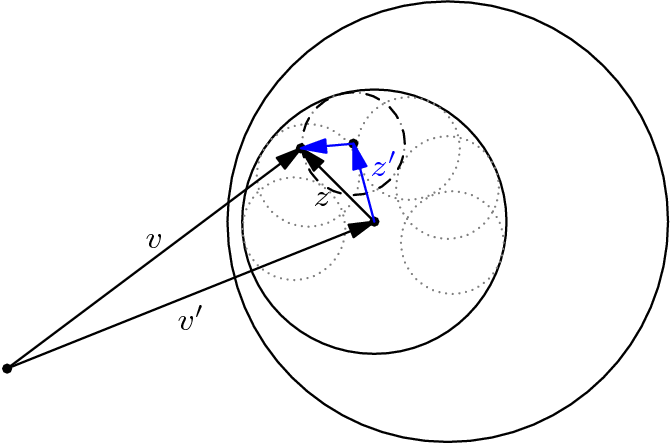
\includegraphics[scale = 0.4]{figures/chaining.png}
    \caption{Illustration of a chained cover. Within the $\epsilon$-ball containing the discretization error $z$, we find a finer $\epsilon'$-cover and obtain a smaller error $z'$ from discretizing $z$.}
    \label{lec8:fig:chained cover}
\end{figure}

Using this method of chaining, we can obtain the following (stronger) result:

\begin{theorem}(Dudley chaining)
Let $\cF$ be a family of functions from $Z$ to $\R$. Then
\begin{equation}
R_S(\cF) \le 12 \int_0^\infty \sqrt{ \frac{\log N(\epsilon, \cF, L_2(p_n))} n } d\epsilon.
\end{equation}
\end{theorem}

We can interpret this bound as removing the discretization error term by averaging over different scales of $\epsilon$. For a proof of this theorem, refer to Theorem 15 of \cite{percynotes}.

	
	%    Include main chapters here.
	%\include{}
	\appendix
	%    Include appendix "chapters" here.
	
	
	%\backmatter
	%    Bibliography styles amsplain or harvard are also acceptable.
	\bibliographystyle{amsalpha}
	\bibliography{bibliography}
	%    See note above about multiple indexes.
%	\printindex
	
	\end{document}
	
	%-----------------------------------------------------------------------
	% End of amsbook-template.tex
	%-----------------------------------------------------------------------
